%
% teil2.tex -- Beispiel-File für teil2 
%
% (c) 2020 Prof Dr Andreas Müller, Hochschule Rapperswil
%
% !TEX root = ../../buch.tex
% !TEX encoding = UTF-8
%
\section{Helmholtz-Zerlegung für $\mathbb{R}^3$
\label{helmholtz:section:teil2}}
\kopfrechts{Teil 2}

Die Grundidee der Helmholtz-Zerlegung besteht darin, dass ein glattes (differenziebares) Vektorfeld $\mathbf{F}$, welches unendlich schnell genug abfällt, in zwei orthogonale Komponenten zerlegenlässt. Und zwar in ein eindeutig wirbelfreien (irrotationalen) Teil und einen quellenfreien (solenoidalen) Teil. Diese Zerlegung spiegelt die physikalischen Eigenschaften des Vektorfeldes wider und ist insbesondere in der Akustik, Strömungsmechanik und Elektrodynamik von zentraler Bedeutung.

\begin{equation}
\underbrace{\mathbf{F}}_{\text{zu zerlegendes Vektorfeld}} =  \underbrace{-\nabla \Phi}_{Skalarpotential} + \underbrace{\nabla \times \mathbf{\Psi}}_{Vektorpotential}
\label{helmholtz:equationAllgemein}
\end{equation}

\begin{itemize}
\item Der erste Term $ \nabla \Phi $ ist wirbelfrei (irrotational), da Rotation verschwindet (Warum genau ???) ($\nabla \times (-\nabla \Phi) = 0$) 
\begin{itemize}
\item Dieser Anteil hat keine Rotation: $\nabla \times (-\nabla \Phi) = 0$
\item Die Feldlinien verlaufen strahlenförmig von Quellen zu Senken
\begin{figure}[htbp]
    \centering
    \begin{subfigure}{}
        \centering
        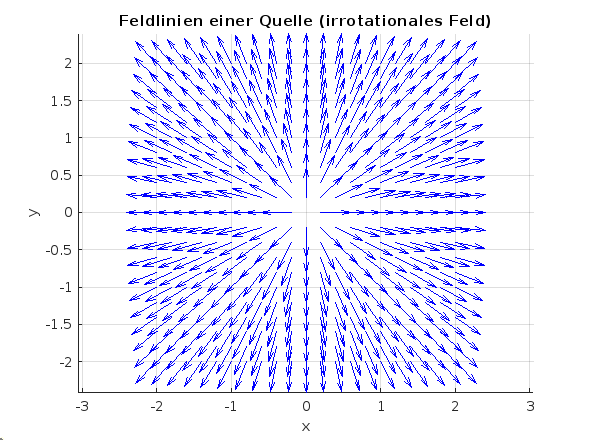
\includegraphics[scale=0.3]{papers/helmholtz/images/Quelle.png}
        \caption{F}
        \label{fig:quelle}
    \end{subfigure}
    \hfill
    \begin{subfigure}{}
        \centering
        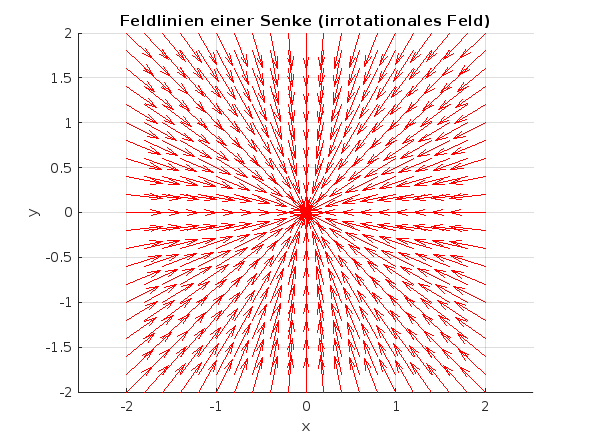
\includegraphics[scale=0.3]{papers/helmholtz/images/Senke.png} 
        \caption{F}
        \label{fig:senke}
    \end{subfigure}
    \caption{}
    \label{fig:vergleich}
\end{figure}
\end{itemize}
\item Der zweite Term $\nabla \times \mathbf{\Psi}$ hat gemäss der Definition immer Divergenz null ($\nabla \cdot (\nabla \times \mathbf{\Psi}) = 0$) und wird auch solenoidal (quellenfrei) genannt. \newline
\begin{itemize}
\item Dieser Anteil hat keine Divergenz:$\nabla \cdot (\nabla \times \mathbf{\Psi}) = 0$
\item Die Feldlinien bilden geschlossene Schleifen (ähnlich einem Magnetfeld).
\end{itemize}
\end{itemize}


\begin{tabular}[h]{l|l|l|l}
\hline
zu zerlegende Vektorfeld & $\mathbf{F}$ & & \\
\hline 
skalares Potential & $\Phi $ & $\nabla \times (-\nabla \Phi) = 0$ & wirbelfrei\\
\hline
Vektorpotential & $\mathbf{\Psi}$ & $\nabla \cdot (\nabla \times \mathbf{\Psi}) = 0$ & quellenfrei\\
\hline
\end{tabular}\newline

Hierzu müssen jedoch die Potentiale $\Phi $ und $\mathbf{\Psi}$ berechnet werden. Dies kann auf verschiedene Methoden gemacht werden abhängig von den Ranbedingungen.

\subsection{Helmholtz-Zerlegung und Komplexe Schallintensität}

Bei näherer Betrachtung ist zu erkennen, dass die Gleichung \eqref{helmholtz:equationAllgemein} dieselbe Struktur wie die Komplexe Schallintensität \eqref{helmholtz:equationIntensitaetKomplex} hat. Somit kann die Zerlegung wie folgt vorgenommen werden

\begin{equation}
\mathbf{I}_c ~(\mathbf{r}) = \underbrace{\mathbf{I}~(\mathbf{r})}_{\text{quellenfrei}} + \underbrace{j\,\mathbf{Q}~(\mathbf{r})}_{\text{wirbelfrei}}
\label{helmholtz:KomplexeIntensitaet_Zerlegung}
\end{equation}

\begin{equation}
\mathbf{I}_c ~(\mathbf{r}) = \underbrace{\mathbf{I}~(\mathbf{r})}_{\nabla \cdot I = 0} + \underbrace{j\,\mathbf{Q}~(\mathbf{r})}_{\nabla \times Q = 0}
\label{helmholtz:KomplexeIntensitaet_Zerlegung}
\end{equation}

\begin{itemize}
\item $\nabla \cdot \mathbf{I} = 0$ aktive Intensität ist quellenfrei
\item $\nabla \times \mathbf{I} = \frac{k}{c} \frac{\mathbf{I} \times \mathbf{Q}}{V}$ aktive Intensität kann wirbel enthalten
\item $\nabla \times \mathbf{Q} = 0$ reaktive Intensität ist wirbelfrei
\item $\nabla \cdot \mathbf{Q} = 2 \omega (T-V)$ reaktive Intensität hat Quellen oder Senken
\end{itemize}


\subsection{Greenscher Ansatz}
Ein möglicher Ansatz, um die partielle Differential Gleichung zu lösen ist der Dirac delta Funktion. Integralform einer Matrixmultiplikation. Es wird die Funktion $\mathbf{F}$, welche in diesem Fall ein Vektor darstellt mit der Deltafunktion multipliziert.

\begin{equation}
\Delta F = -4 \pi \rho 
\label{helmholtz:DGL_idee}
\end{equation}

\begin{equation}
\underbrace{\frac{1}{4 \pi} \Delta F}_{invertiert} = \rho 
\label{helmholtz:DGL_idee_umformung}
\end{equation}

\begin{tabular}{ll}
  & Idee in Matrix \\
$\Delta F = -4 \pi \rho$  & $Au = f$ \\
$\underbrace{\frac{1}{4 \pi} \Delta F}_{invertiert} = \rho$ & $A^{-1}Au = A^{-1}f$  \\
s & $u = A^{-1}f$  \\
\end{tabular}

\begin{equation}
\delta (\mathbf{x} - \mathbf{x'}) = \frac{1}{4 \pi} \nabla^2 \frac{1}{|\mathbf{x} - \mathbf{x'}|}
\label{helmholtz:dirac}
\end{equation}

Einheitsmatrix mal Vektor gleich Matrix. 



\begin{equation}
\mathbf{F}(\mathbf{r}) = -\frac{1}{4\pi} \int_V \mathbf{F}(\mathbf{r}') \nabla^2 \left( \frac{1}{|\mathbf{r} - \mathbf{r}'|} \right) dV'
\end{equation}

Die Identität

\begin{equation}
\nabla^2 \mathbf{\Psi}= \underbrace{\nabla \Big( \nabla \cdot \mathbf{\Psi} \Big)}_{\text{Gradient}} -\underbrace{\nabla \times \Big(\nabla \times \mathbf{\Psi} \Big)}_{\text{Rotation}}
\end{equation}

Das Vektorfeld $\mathbf{F}$ kann nun geschrieben werden als:

\begin{equation}
\mathbf{F}(\mathbf{r}) = - \frac{1}{4 \pi} \nabla \bigg( \nabla \cdot \int_V \frac{\mathbf{F}(\mathbf{x}^{\prime})}{|\mathbf{r} - \mathbf{r}^{\prime}|} d\mathbf{x}^{\prime} \bigg) + \frac{1}{4 \pi} \nabla \times \bigg( \nabla \times \int_V \frac{\mathbf{F}(\mathbf{x}^{\prime})}{|\mathbf{r} - \mathbf{r}^{\prime}|} d\mathbf{x}^{\prime} \bigg)
\end{equation}


\subsection{Bedingungen
\label{helmholtz:subsection:Bedingung}}

Damit die Zerlegung vorgenommen werden kann bzw. darf, muss das Vektorfeld $\mathbf{A}$ 

\begin{itemize}
\item \textbf{Glatt sein:} $\mathbf{A}$ stetig/kontinuirlich differenziebar sein (in $\mathbb{R}^3$ 2 mal differenziebar) in dem Gebiet
\item \textbf{Abfallverhalten:} $\mathbf{A}$ schnell abfallen  $\mathbf{A}$ schneller als $1/r$. 
\end{itemize}
(Unsicher bei dieser Aussage. Formel?)

%https://www.youtube.com/watch?v=RVlUe5gsAX4
%https://icmp.lviv.ua/journal/zbirnyk.89/13002/art13002.pdf

\subsection{Berechnung der Potentiale unbeschränkte Gebiete
\label{helmholtz:subsection:Berechnung}}

%https://people.iith.ac.in/ashok/Maths_Lectures/TutorialB/Topic_03_(Helmholtz%27%2520Theorem).pdf

Berechnung der Potentiale $\Phi $ und $\mathbf{\Psi}$ lassen sich mit Hilfe der Greenschen Funktion herleiten. Wer Wie Wo Was?


\begin{itemize}
\item \textbf{skalares Potential}
\begin{equation}
\phi = \frac{1}{4 \pi} \int_{V} \frac{\nabla \cdot \mathbf{A}}{\mu}, dV
\end{equation}
\item \textbf{Vektorpotential}
\begin{equation}
\mathbf{\Psi} = \frac{1}{4 \pi} \int_{V} \frac{\nabla \times \mathbf{A}}{\mu}, dV
\end{equation}
\item $\vec{\mu} = \mid \vec{r} - \vec{r}^{\prime} \mid$ was ist das genau?
\end{itemize}

\subsection{Berechnung der Potentiale beschränktem Gebiet
\label{helmholtz:subsection:BerechnungBeschr}}

endliches (beschränktes) Volumen $V$ Oberflächenintegrale ?

\begin{itemize}
\item \textbf{skalares Potential}
\begin{equation}
\Phi (\mathbf{r}) = \frac{1}{4\pi} \int_V \frac{\nabla' \cdot \mathbf{F}(\mathbf{r}')}{|\mathbf{r} - \mathbf{r}'|} dV' + \frac{1}{4\pi} \oint_S \frac{\mathbf{F}(\mathbf{r}')}{|\mathbf{r} - \mathbf{r}'|} dxXx'
\end{equation}
\item \textbf{Vektorpotential}
\begin{equation}
\mathbf{\Psi}(\mathbf{r}) = \frac{1}{4\pi} \int_V \frac{\nabla' \times \mathbf{F}(\mathbf{r}')}{|\mathbf{r} - \mathbf{r}'|} dV' + \frac{1}{4\pi} \oint_S \frac{\mathbf{F}(\mathbf{r}')}{|\mathbf{r} - \mathbf{r}'|} dxXx'
\end{equation}
\end{itemize}


\subsection{Eindeutigkeit der Zerlegung 
\label{helmholtz:subsection:EindeutigkeitS}}

\begin{itemize}
\item \textbf{Für unbeschränkte Gebiete}
\item \textbf{Für beschränkte Gebiete}
\end{itemize}


\subsection{Orthogonalität
\label{helmholtz:subsection:Orthogonalitaet}}

